\documentclass{article}
\usepackage[T1]{fontenc}
\usepackage{lmodern}
\usepackage{graphicx}
\usepackage{amsmath,amssymb}
\usepackage[a4paper,margin=2cm]{geometry}
\usepackage[absolute,overlay]{textpos}
\setlength{\TPHorizModule}{1mm}
\setlength{\TPVertModule}{1mm}
\usepackage[indonesian]{babel}
\usepackage{hyperref}
\setlength{\emergencystretch}{2em}
% unit: Halaman 45

\begin{document}

% === Halaman 45 (llm) ===

3. Lakukan pengacakan (permutasi) nilai-nilai di dalam larik S berdasarkan kunci rahasia K (kunci eksternal dari pengguna):

\vspace{5mm}

\begin{itemize}
    \item Permutasi ini menyebabkan elemen-elemen di dalam larik S teracak.
    \item $\text{K[i mod Length(K)]}$ menyatakan karakter-karakter kunci diulang secara periodik jika panjangnya kurang dari 256
\end{itemize}

% deskripsi: Potongan kode pseudocode untuk melakukan permutasi pada larik S menggunakan kunci K.
% bbox normalisasi: [0.1480, 0.2940, 0.8670, 0.5810]
\begin{textblock*}{150.99mm}(31.08mm,87.32mm)
\noindent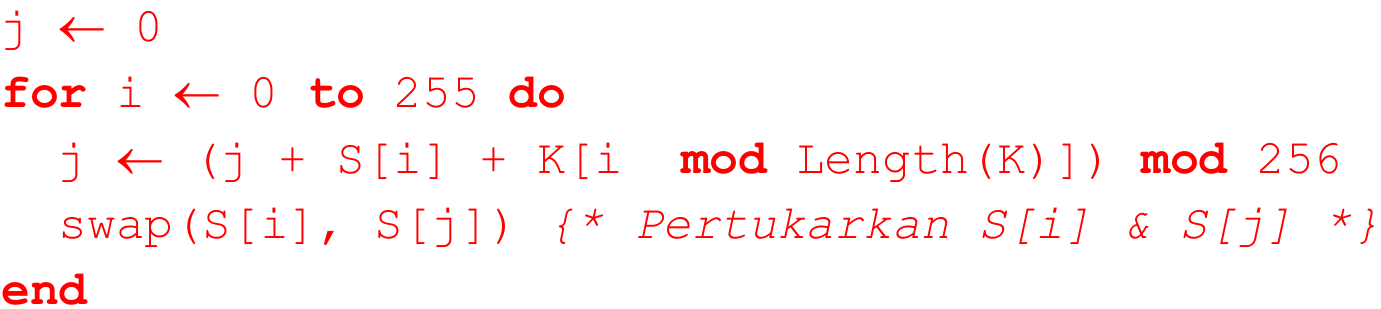
\includegraphics[width=150.99mm,height=85.24mm]{../../images/llm/page_045_img_01.png}%
\end{textblock*}

\end{document}
